\chapter{Aims and Objectives}

This chapter will discuss the program which shall be implemented.
To do so, the problem to solve must be understood.
To gather requirements and understand the technical hurdles to overcome, this chapter is split into two sections.
First, a rough glance over the current workflow is given, which is followed by a more detailed description for the desired workflow.


\section{Current Workflow}

Currently, to analyze a video for the trajectories of  recorded vehicles, the following steps are executed manually:
\begin{enumerate}
	\item Upload the input video to a new directory on the GPU server
	\item \label{cw:ex} Execute a shell script with the video as input file and let it run (hours to days) until completed. The shell script invokes a Java Program - called TrackerApplication - with parameters on what to do with the input file and additional parameters.
	\item The intermediate result with raw detection results is downloaded to the local machine and opened for inspection. If the detection error is too high, the camera tracking has a drift or other disruptions are visible, the previous step is redone with adjusted parameters.
	\item \label{cw:st} Upload the video and intermediate result to a generic computing server and run data cleanup and analysis. This is achieved with the same Java Program as in step \ref{cw:ex}, but with different stage environment parameters.
	\item \label{cw:st_dl} Download the results, recheck for consistency or obvious abnormalities. Depending on the result, redo step \ref{cw:ex} or \ref{cw:st} with adjusted parameters again.
	\item Depending on the assignment, steps \ref{cw:st} and \ref{cw:st_dl} are repeated to incrementally accumulate all output data (such as statistics, diagrams and so on).
\end{enumerate}

Because all those steps are done manually, the user needs to check for errors by oneself.
Also, if a execution is finished or has failed early, there could be hours wasted until noticed, if the check intervals are too far apart, such as during nights or weekends.

\begin{figure}[H]
	\centering
	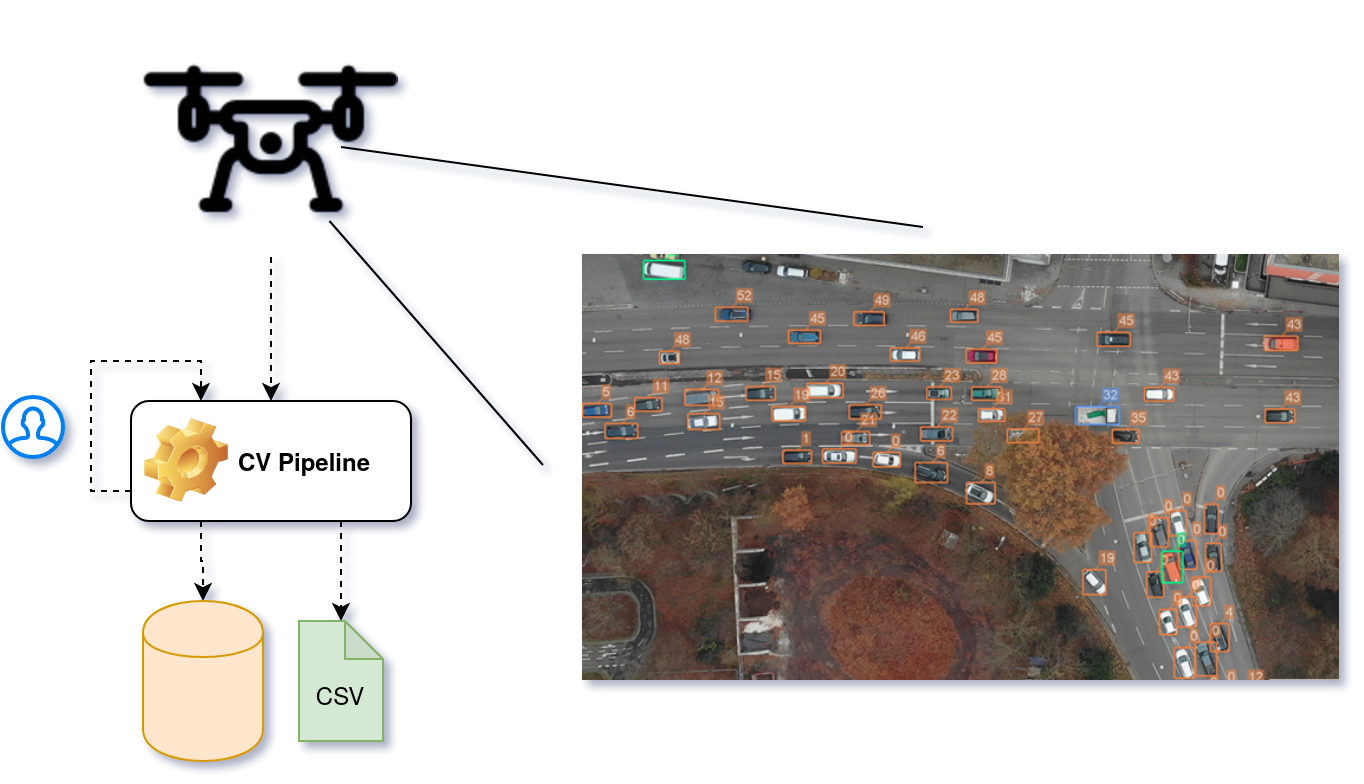
\includegraphics[width=0.9\textwidth]{overview_3.png}
	\caption{Overview of workflow}
\end{figure}

\section{Desired Workflow}
\label{workflow}
\label{workflow:desired:docker}

The desired workflow shall be supported through an user interface that provides an overview of all active projects and their current state, such as running computation, awaiting user input, failed or succeeded.

To create a new project, a predefined pipeline definition shall be selected as well as a name chosen.
Because only a handful of different pipeline definitions are expected, the creation of such does not need to happen through the user interface.
Instead, it is acceptable to have to manually edit a configuration file in such rare circumstances.

Once a project is created, the user wants to select the path to the input video.
This file has to be been uploaded to a global resource pool at this point.
The upload and download of files shall therefore also be possible through the user interface.
Because a video is usually recorded in 4k (3840 x 2160 pixels), encoded with H.264 and up to 20 minutes long, the upload must be capable of handling files which are tens of gigabytes large.

Once a pipeline is started, it shall execute the stages on the most fitting server node until finished, failed or a user input is required.
Throughout, the logs of the current and previous stage shall be accessible as well as uploading or downloading files from the current or previous stages workspace.
In addition to the pipeline pausing itself for user input, the user shall be able to request the pipeline to pause after the current stage at any moment.
When resuming the pipeline, the user might want to overwrite the starting point to, for example, redo the latest stage.

Mechanisms for fault tolerance shall detect unexpected program errors or failures of server nodes.
Server nodes shall be easily installed and added to the existing network of server nodes.
Each server node might provide additional hardware (such as GPUs), which shall be detected and provided.

For the ease of installation and binary distribution, Docker Images shall be used for running the Java Program for analyzing the videos as well the to be implemented management software.

%\todo{describe: project/pipeline -> stage?}




\section{Deliverable Requirements}

From the desired workflow, the following requirements can be extracted:

\begin{itemize}
	\item User interface for interaction between the system and the user
	\item Storage management for global resource files as well as stage based workspaces
	\item Pipeline definition through configuration files
	\item Handling of multiple projects with independent progress and environment
	\item Reflecting the correct project state (running, failed, succeeded, paused)
	\item Log accumulation and archiving
	\item Accepting user input to update environment variables, resuming and pausing projects as well as uploading and downloading files into or from the global resource pool or a stages workspace.
	\item Assigning starting stages to the most fitting server node
	\item Detecting program errors (in a stage execution)
	\item Cope with server node failures
	\item Providing a Docker Image for the implemented program, preferably in an automated fashion.
\end{itemize}

Furthermore, a given constraint is that the user interface is to be implemented as Angular Web-Application using a REST API (for more details see \autoref{fundamental:angular}).

\todo{mention? node failure resilient, easy to setup, decentralized?}

%\todo{something something agile extended as needed? \autoref{fundamental:agile}}

\begin{comment}
\subsection{Derived Requirements} \todo{.}
Requirements that are derived by looking at other requirements.


\todo{functional vs nonfunctional}

Die hier gelisteten funktionalen Anforderungen beschreiben das gewünschte Verhalten des
Systems \cite[155]{goll2012methoden}.

Nichtfunktionale Anforderungen zeigen im Gegensatz zu funktionalen Anforderungen Rah-
menbedingungen bei der Umsetzung des Systems auf \cite[155]{goll2012methoden}.
\end{comment}


\subsection{Non-Requirements}

To know the requirements and expectations of a system is essential, but knowing what is not expected by the system is at least as valuable.
It prevents wasting resources, effort and architectural specialization that will never be required or in the worst case, make further development harder by restricting available choices in the future.
 
The system to implement shall not strive to implement real time scheduling or low latency scheduling.
The expected work items are big chunks that require hours to compute.
Whether the assignment of the work item takes sub seconds or several seconds is nearly unnoticeable in the overall compute time.